\documentclass[]{article}
\usepackage[utf8]{inputenc}
\usepackage{polski}
\usepackage{listings}
\usepackage[usenames,dvipsnames]{xcolor}
\usepackage{geometry}
\usepackage{subcaption}
\usepackage{graphicx}
\usepackage{amsmath}
\usepackage{amssymb}
\usepackage{hyperref}
\usepackage{enumerate}
\usepackage{tabularx}
\usepackage{multirow,bigdelim}
\usepackage[font=small]{caption}
\usepackage[ruled,noend]{algorithm2e}
\usepackage{bm}
\SetAlgorithmName{Algorytm}{algorytm}{Algorytmy}
\DeclareGraphicsExtensions{.png}
\graphicspath{ {./} }
\geometry{
	a4paper,
	left=25mm,
	right = 25mm,
	top=20mm,
	bottom=20mm
}
%%\hyphenchar\font=-1

\title{
	Sprawozdanie \\
	\large 
	Obliczenia naukowe - lista 5}
\author{Kamil Król}
\date{244949}
\newcommand{\mA}{\bm{A}}
\newcommand{\mB}{\bm{B}}
\newcommand{\mC}{\bm{C}}
\newcommand{\mL}{\bm{L}}
\newcommand{\mU}{\bm{U}}
\newcommand{\mZ}{\bm{0}}
\newcommand{\vb}{\bm{b}}
\newcommand{\vx}{\bm{x}}
\newcommand{\R}{\mathbb{R}}

\begin{document}
	
	\maketitle
	
	\section*{Opis problemu oraz struktury danych}
	Celem listy jest rozwiązanie układu równań liniowych: 
	$\mA\vx = \vb$,
	dla danej macierzy $\mA \in \R^{n\times n}$ 
	i wektora prawych stron $\vb \in \R^n$, gdzie $n \geq 4$. \\
	
	\noindent Zgodnie z treścią listy macierz $\mA$ jest rzadką macierzą (tj. mającą dużo elementów zerowych) blokową o następującej strukturze:
	$$
	\mA =
	\left(\begin{array}{ccccccc}
	\mA_1 & \mC_1 & \mZ & \mZ & \mZ & \cdots & \mZ \\
	\mB_2 & \mA_2 & \mC_2 & \mZ & \mZ  & \cdots & \mZ \\
	\mZ  & \mB_3 & \mA_3 & \mC_3 & \mZ  & \cdots & \mZ \\
	\vdots & \ddots & \ddots & \ddots & \ddots & \ddots & \vdots\\
	\mZ   & \cdots & \mZ  & \mB_{v-2} & \mA_{v-2} & \mC_{v-2} & \mZ \\
	\mZ  & \cdots & \mZ  &  \mZ &\mB_{v-1} & \mA_{v-1} & \mC_{v-1}  \\
	\mZ  & \cdots & \mZ & \mZ & \mZ& \mB_{v} & \mA_{v}  \\
	\end{array}\right),
	$$
	$v = n/\ell$, zakładając że $n$ jest podzielne przez $\ell$, gdzie $\ell \geq 2$ jest rozmiarem wszystkich kwadratowych macierzy wewnętrznych (bloków) $\mA_i$, $\mB_i$, $\mC_i$, $\mZ$. \\
	
	\noindent Macierze oznaczone przez $\mZ$ są macierzami zerowymi tzn. $\mZ \in \R^{\ell\times \ell}$. Macierze $\mA_i$, $\mB_i$, $\mC_i$, są następującej postaci:
	\begin{enumerate}[(i)]
		\item $\mA_i \in \R^{\ell\times \ell}$,   $i = 1, \ldots,v$ -- macierze gęste,
		\item $\mB_i \in \R^{\ell\times \ell}$,   $i = 2, \ldots,v$ -- macierze mające tylko dwie ostatnie kolumny niezerowe:
		$$
		\mB_i =
		\left(\begin{array}{ccccc}
		0 & \cdots & 0 & b_{1\,\ell-1}^i & b_{1\,\ell}^i \\
		0 & \cdots & 0 & b_{2\,\ell-1}^i & b_{2\,\ell}^i \\
		\vdots & & \vdots & \vdots & \vdots \\
		0 & \cdots & 0 & b_{\ell\,\ell-1}^i & b_{\ell\,\ell}^i \\
		\end{array}\right),
		$$
		\item $\mC_i \in \R^{\ell\times \ell}$,   $i = 1, \ldots,v\!-\!1$ -- macierze diagonalne:
		$$
		\mC_i =
		\left(\begin{array}{ccccc}
		c_{1}^i & 0 & 0 & \cdots & 0  \\
		0 &  c_{2}^i &  0 & \cdots & 0  \\
		\vdots &  \ddots &  \ddots & \ddots & \vdots  \\
		0 & \cdots & 0 &  c_{\ell-1}^i & 0 \\
		0 & \cdots & 0 &  0 & c_{\ell}^i \\
		\end{array}\right).
		$$
	\end{enumerate}

	Dodatkową informacją o danych jest ich duży rozmiar. W konsekwencji wyklucza to pamiętanie macierzy $\mA$ jako tablicę o wymiarach $n \times n$ oraz użycie standardowych (bibliotecznych) algorytmów dla macierzy gęstych tj. takich, gdzie
	nie zakłada się dużej liczby elementów zerowych. Zatem dodatkowym wymaganiem co do zadania jest specjalna struktura pamiętająca efektywnie macierz $\mA$. Taka, która pamięta tylko elementy niezerowe macierzy $\mA$. W tym celu w moich programach użyłem biblioteki \textit{SparseArrays}, która pamięta tylko elementy niezerowe. W naszych rozważaniach założymy, że możemy uzyskać dostęp do elementów macierzy w czasie stałym -- $O(1)$. W rzeczywistości tak nie jest. \\
	Samo użycie tej biblioteki jednak nie gwarantuje nam szybkiego algorytmu. Pojawia się bowiem problem w momencie nadpisywania elementów macierzy, które są zerami. W momencie takiego przypisania konieczna jest alokacja dodatkowej pamięci aby przechować nowy niezerowy element. Jedną z kluczowych optymalizacji, którą zastosujemy będzie sztuczne przypisanie zer do \textit{pól} macierzy $\mA$ w obszarach gdzie zera faktycznie występują, ale zostaną one w przyszłości nadpisane. Takie obszary to obszary macierzy $\mC$ poza elementami na diagonali. Zastosowanie tej optymalizacji pozwoliło aby wykresy przedstawiające czas wykonywania algorytmów od wielkości macierzy, które są przedstawione na końcu sprawozdania, faktycznie przypominały liniowe.\\
	Ponadto konieczna jest modyfikacja standardowych algorytmów tak, aby uwzględniały one specyficzną postać macierzy $\mA$, tj.
	jej rzadkość, regularność występowania elementów zerowych i niezerowych.\\
	
	\noindent Zaimplementowane przeze mnie algorytmy (napisane w języku Julia i opisane poniżej) działają na macierzy transponowanej, ze względu na optymalizację tzn. dostęp do elementów po kolumnach jest szybszy niż po wierszach. W dalszych rozważaniach pominiemy ten fakt gdyż transpozycja nie zmienia wewnętrznej struktury macierzy $\mA$ oraz nie zmienia ogólnej idei algorytmu.
	Odnośnik do dokumentacji: 
	\href{https://docs.julialang.org/en/v1/stdlib/SparseArrays/}{julialang - SparseArrays}.
	

	\section*{Opis metody eliminacji Gaussa bez wyboru elementu głównego}
	Ideą eliminajci Gaussa jest to aby początkowy układ równań sprowadzić do układu prostszego. Dokładniej chodzi o sprowadzenie macierzy A do postaci macierzy trójkątnej górnej. W celu doprowadzenia macierzy do takiej postaci, algorytm posługuje się podstawowymi operacjami na macierzy tzn. dodawanie, odejmowanie wierszy oraz mnożenie wierszy przez pewnien niezerowy współczynnik. \\
	Dokładniej, proces polega na eliminowaniu (zerowaniu) elementów znajdujących się w pod przekątną macierzy.
	Zatem dla kolumny pierwszej będziemy chcieli wyzerować wszystkie elementy znajdujące się pod pierwszym elementem w tej kolumnie, dla kolumny drugiej -- wszystkie elementy pod drugim (patrząc od góry) elementem w danej kolumnie. Bardziej formalnie, naszym celem będzie wyeliminowanie niewiadomej $x_1$ ze wszystkich $n-1$ pozostałych równań (czyli wszystkich poza pierwszym). Dla $i = 2,\ldots,n$ będziemy odejmować odpowiednią wielokrotność równania pierwszego od $i$-tego równania zerując przy tym współczynnik przy $x_1$ w $i$-tym równaniu. \\
	Ogólnie dla macierzy A i jej elementów $a_{ij}$, gdzie $i,j = 1,\ldots,n$ i dla jej $k$-tej kolumny, będziemy zerować wszystkie elementy poniżej elementu na przekątnej w tej kolumnie, czyli $a_{kk}$. Dla $i = k+1,\ldots,n$ będziemy odejmować odpowiednią wielokrotność równania $k$-tego od $i$-tego równania zerując przy tym współczynnik przy $x_k$ w $i$-tym równaniu. Inaczej aby wyzerować to $x_k$ będziemy musieli pomnożyć wiersz $k$ przez pewien współczynnik $\psi_{ik}$, króty dalej będziemy nazywać mnożnikiem, a następnie odjąć go od $i$-tego wiersza. Łatwo zauważyć, że mnożnik ten możemy obliczyć, ze wzoru $\psi_{ik}$ = $\frac{a_{ik}}{a_{kk}}$. Widać też, że w przypadku kiedy na diagonali pojawi się element równy zero nasz algorytm nie zadziała, ponieważ pojawi się konieczność dzielenia przez zero. \\
	Zanim zobaczymy jak można rozwiązać ten problem musimy przytoczyć jedną z własności układu równań Ax=b. Mianowicie, wiersze macierzy A i odpowiadające im wartości w wektorze b możemy dowolnie ze sobą zamieniać. Nie zmianiamy w ten sposób układu równań.
	Zwróćmy również uwagę na fakt, że aby istniało rozwiązanie tego równania macierz A musi być nieosobliwa. 
	Teraz możemy przedstawić sposób na uniknięcie dzielenia przez 0. 
	\clearpage
	\section*{Opis metody eliminacji Gaussa z częściowym wyborem elementu głównego}
	Przedstawiona poniżej metoda nosi nazwę metody eliminacjii Gaussa z częściowym wyborem elementu głównego.
	Czym jest element główny? Jest to element macierzy znajdujący się na diagonali. Dla $k$-tej kolumny, elementem głównym będzie element $a_{kk}$ macierzy A. Jest to również ten element przez który dzielimy chcąc obliczyć mnożnik $\psi_{ik}$ ($k$ oraz $i$ są opisane tak samo jak w poprzednim paragrafie). Częściowy wybór polega na wybraniu największego elementu co do wartości bezwzględnej z danej kolumny $k$ oraz zamianie wierszy tak aby ten element stał się elementem głównym -- elementem na diagonali. Możemy to zrobić, ponieważ macierz A jest nieosobliwa. \\
	Zamiana wierszy macierzy jest kosztownym procesem, który może być zastąpiony przez wektor permutacji wierszy $p$. Zapamiętujemy w nim, na którym miejscu aktualnie znajduje się dany wiersz. Zatem jedyna różnica w samym algorytmie będzie taka, że zamiast odwoływać się do danego wiersza bezpośrednio, będziemy się odwoływać do jego pozycji zapisanej w wektorze permutacji. Zwróćmy uwagę na to, że zmieniając wiersze w macierzy A musimy zmieniać też poszczególne współrzędne w wekotrze prawych stron -- b. Złożoność obu przedstawionych powyżej algorytmów wynosi $O(n^3)$.
	
	Teraz kiedy znamy procedurę, która pozwala nam sprowadzić macierz A do macierzy trójkątnej górnej, pojawia się pytanie jak z tą wiedzą rozwiązać układ równań $Ax = b$. W tym celu zastosujemy algorytm podstawiania wstecz. Opiera się on o wzór poniżej.
	$$x_i = \frac{b_i - \sum_{j = i+1}^n (a_{ij} \cdot x_j)}{a_{ii}}$$
	
	Widać zatem, że idąc \textit{od końca} ($i=n,\ldots,1$) jesteśmy w stanie obliczyć wszystkie wartości $x$. Złożoność tego algorytmu wynosi $O(n^2)$, a cały proces prowadzący do rozwiązania równania ma złożoność $O(n^3)$ (bo eliminacja Gaussa ma złożoność $O(n^3)$). \\
	Widać tu, że najkosztowniejszym fragmentem opisanego wyżej algorytmu rozwiązywania układu równań jest eliminacja Gaussa. Przedstawiony poniżej rozkład LU będzie umożliwiał rozwiązywanie układu równań dla różnych wektorów prawych stron przy tylko jednym wywołaniu metody eliminacji Gaussa zajmującej $O(n^3)$. Rozwiązywanie kolejnych układów równań z tą samą macierzą A będzie robione w czasie $O(n^2)$.
	\clearpage
	\section*{Zadanie 1}
	
	Celem tego zadania było napisanie funkcji rozwiązującej układ $\mA\vx = \mB$ metodą eliminacji Gaussa uwzględniającej specyficzną postać macierzy $\mA$ dla dwóch wariantów:
	\begin{enumerate}[a)]
		\item bez wyboru elementu głównego,
		\item z częściowym wyborem elementu głównego.
	\end{enumerate}

	Znając wyżej opisane algorytmy należało zmodyfikować je pod opisaną w treści listy zadań strukturę. Wiemy, że rozwiązanie naszego równania z użyciem niezmodyfikowanych algorytmów ma złożoność $O(n^3)$. Celem jest zrobienie tego samego w czasie $O(n)$. Zakładamy tu, że rozmiar bloku $\ell$ jest stałą. Inne założenie opisane wyżej to założenie, że dostęp do elementu macierzy (Sparse Arrays) jest w czasie stałym.\\
	\textbf{Zastosowane modyfikacje}\\
	Macierz $\mA$ jest macierzą rzadką o specyficznej blokowo-trójdiagonalnej strukturze. Oznacza to, że większość elementów w danej kolumnie nie będzie wymagało zerowania. Znana i uporządkowana struktura pozwala nam na ograniczenie ilości wykonywanych operacji, gdyż są one wymagane tylko dla pewnego ograniczonego obszaru macierzy $\mA$. Wyznaczymy teraz te ograniczenia. W celu przedstawienia metody rozważmy macierz $\mA$ dla $\ell = 4$ i jakiegoś $n$.
$$
	\mA =
	\left(\begin{array}{cccccccccccccc}
	a^1_{11} & a^1_{12} & a^1_{13}  & a^1_{14} & c^1_{11} & 0  & 0  & 0 & 0  & 0  & 0  & 0  & \cdots  \\
	a^1_{21} & a^1_{22} & a^1_{23}  & a^1_{24} & 0 & c^1_{22} & 0  & 0  & 0  & 0  & 0  & 0  & \cdots  \\
	a^1_{31} & a^1_{32} & a^1_{33}  & a^1_{34} & 0  & 0  &  c^1_{33} & 0 & 0  & 0  & 0  & 0  & \cdots  \\
	a^1_{41} & a^1_{42} & a^1_{43}  & a^1_{44} & 0  & 0  & 0 & c^1_{44} & 0  & 0  & 0  & 0  & \cdots   \\
	0 & 0 & b^2_{13}  & b^2_{14} & a^2_{11} & a^2_{12} & a^2_{13}  & a^2_{14} & c^2_{11} & 0  & 0  & 0 &\cdots& \\
	0 & 0 & b^2_{23}  & b^2_{24} & a^2_{21} & a^2_{22} & a^2_{23}  & a^2_{24} & 0 & c^2_{22} & 0  & 0  &\cdots &\\
	0 & 0 & b^2_{33}  & b^2_{34} & a^2_{31} & a^2_{32} & a^2_{33}  & a^2_{34} & 0  & 0  &  c^2_{33} & 0&\cdots &\\
	0 & 0 & b^2_{43}  & b^2_{44} & a^2_{41} & a^2_{42} & a^2_{43}  & a^2_{44} & 0  & 0  & 0 & c^2_{44} &\cdots &\\
	0&0&0&0&0&0& b^3_{13}  & b^3_{14} & a^3_{11} & a^3_{12} & a^3_{13}  & a^3_{14} &\cdots \\
	0&0&0&0&0&0& b^3_{23}  & b^3_{24} & a^3_{21} & a^3_{22} & a^3_{23}  & a^3_{24} &\cdots \\
	0&0&0&0&0&0& b^3_{33}  & b^3_{34} & a^3_{31} & a^3_{32} & a^3_{33}  & a^3_{34} &\cdots \\
	0&0&0&0&0&0& b^3_{43}  & b^3_{44} & a^3_{41} & a^3_{42} & a^3_{43}  & a^3_{44} &\cdots \\
	\vdots & \vdots &\vdots &\vdots &\vdots &\vdots &\vdots &\vdots &\vdots &\vdots &\vdots &\vdots & \ddots \\
	\end{array}\right)
$$

	Kiedy przyjrzymy się czterem ($\ell$) pierwszym kolumnom, widzimy, że musimy w nich wyzerować kolejno 3, 2, 1+4, 0+4 elementów. Zatem pętla która \textit{idzie} po wierszach danej kolumny będzie mogła zakończyć pracę wcześniej. W naszym przypadku na rysunku, w przypadku kolumny pierwszej, pętla będzie mogła zakończyć pracę już po 3 iteracjach, ponieważ wszystkie elementy poniżej $a^1_{41}$ są już zerami.
	Ogólnie jeśli przyjrzymy się $\ell -2$ pierwszym kolumnom to możemy zauważyć, że jedyne elementy niezerowe występują w bloku $\mA_1$, a więc tylko w $\ell$ pierwszych wierszach. Rozpatrując kolejne $\ell$ kolumn widać, że niezerowe elementy będą się znajdować w bloku $\mB_2$ lub $\mC_1$, lub w bloku $\mA_2$, a więc poniżej tych bloków, czyli poniżej wiersza o numerze $2\ell$, nie pojawią się żadne elementy niezerowe. Biorąc kolejne $\ell$ kolumn sytuacja jest podobna -- elementy niezerowe wystąpią \textbf{najniżej} w bloku $\mB_3$ lub $\mA_3$, a więc nie niżej niż wiersz o numerze $3\ell$ licząc od góry ($3\ell$ pierwszych wierszy). Patrząc na przedstawioną wyżej zależność możemy wywnioskować wzór na ostatni element niezerowy w danej kolumnie $k$. 
	$$ ostatni_{wiersz}(k) = min\lbrace \ell + \ell \times \lfloor \frac{k+1}{\ell}\rfloor , n \rbrace, k - \text{indeks kolumny} $$
	Kolejna obserwacja to fakt, że podczas odejmowania wiersza z elementem głównym od innego wiersza nie musimy obliczać tych elementów dla których wiersz główny ma zera. Niech wiersz $k$ będzie naszym wierszem głównym (czyli tym zawierającym element główny), a obecnie eliminowany element będzie w wierszu $i$-tym. Oznacza to, że wykonujemy działanie na wierszach $ R_i \leftarrow R_i -\psi_{ik} \cdot R_k$, gdzie $R_i$ i $R_k$ to odpowiednio $i$-ty i $k$-ty wiersz, a $\psi_{ik}$ to mnożnik (przedstawiony w opisie podstawowej metody eliminacji Gaussa). Teraz widać, że dla $j$-tego elementu wiersza $R_k$ będącego zerem, nazwijmy go $r^k_j = 0$, wykonanie powyższego działania nie zmieni odpowiedniej wartości $j$-tego elementu wiersza $R_i$. Wynika z tego, że pętla która wykonuje to działanie na wierszach może skończyć wcześniej pracę. Teraz wyprowadzimy wzór na ostatnią kolumnę, która może zawierać niezerowy element.\\
	Zauważmy, że ostatnie elementy w wierszach to te leżące na diagonali bloków $\mC$. Są one odległe od diagonali macierzy $\mA$ o dokładnie $\ell$. Zatem ostatni element niezerowy w wierszu $w$ będzie się znajdował w kolumnie o indeksie $min\lbrace \ell + w , n \rbrace $. Podsumowując:
	$$ ostatnia_{kolumna}(w) = min\lbrace \ell + w , n \rbrace, w - \text{indeks wiersza} $$
	Udało się zatem określić ograniczenia pętli w metodzie eliminacji Gaussa, które znacznie zredukują liczbę wykonywanych operacji. Kolejny etap rozwiązywania układu równań to algorytm podstawiania wstecz, który również może zostać zmodyfikowany w celu redukcji wykonywanych operacji.\\
	W algorytmnie tym sumujemy elementy w danym wierszu pomnożone przez pewne liczby. My jednak wiemy, że znaczna część z tych elementów jest zerami, a więc wyniki iloczynów które otrzymamy też będą zerami nie zmianiając tym wartości sumy. Ponadto wiemy na jakiej pozycji występuje ostatni element niezerowy. Jest to zależność wyprowadzona powyżej tzn. wzór na $ostatnia_{kolumna}$. Możemy zatem zakończyć pętlę wcześniej redukując tym liczbę operacji.\\
	Poniżej znajduje się pseudokod omówionego algorytmu w celu podsumowania naszych rozważań.
\begin{algorithm}[h]
	\DontPrintSemicolon
	\SetKwInOut{Input}{Dane wejściowe}
	\SetKwInOut{Output}{Dane wyjściowe}
	\SetKwProg{Fn}{function}{}{}
	\SetKw{KwDownTo}{downto}
	\SetKw{Err}{error}
	
	\SetKwData{L}{$\ell$} 			
	\SetKwData{N}{$n$}    				
	\SetKwData{B}{$\vb$}    		
	\SetKwData{A}{$\mA$}    			
	\SetKwData{X}{$\vx$}
	\SetKwData{F}{f}
	\SetKwData{Z}{$\psi$}
	\SetKwData{I}{i}
	\SetKwData{J}{j}
	\SetKwData{K}{k}
	\SetKwData{Sum}{suma}
	\SetKwData{Col}{$ostatnia_{kolumna}$}
	\SetKwData{Row}{$ostatni_{wiersz}$}
	\SetKwFunction{ge}{eliminacja\_gaussa}
	\SetKwFunction{Min}{$\min$}
	
	\Input{\\
		\begin{tabularx}{0.85\linewidth}{rcX}
			{\A} & -- & macierz z zadania o opisanej w zadaniu strukturze,\\
			{\B} & -- & wektor prawych stron, \\
			{\N} & -- & rozmiar macierzy \A, \\
			{\L} & -- & rozmiar bloku macierzy \A.  		
		\end{tabularx}
	}
	\Output{\\
		\begin{tabularx}{0.85\linewidth}{rcX}
			{\X}& -- & wektor zawierający rozwiązania układu $\A\X=\B$.
		\end{tabularx}					    			
	}
	\Fn{\ge{\A,~\B,~\N,~\L}}{
		\For{$\K \gets 1$ \KwTo $\N-1$} {
			$\Row\gets\Min\lbrace \L + \L \cdot \left \lfloor\frac{\K + 1}{\ell}\right \rfloor, n \rbrace$\;
			$\Col\gets \Min\lbrace\K + \L, \N\rbrace$\;
			\For{$\I \gets \K+1$ \KwTo \Row}{
				\If{$\A[\K,\K] = 0$}{\Err współczynnik na przekątnej równy zero}
				$\Z \gets \frac{\A[\I,\K]}{ \A[\K,\K]} $\;
				$\A[\I,\K] \gets 0 $ \;
				\For{$\J \gets \K+1$ \KwTo \Col}{
					$\A[\I,\J] \gets \A[\I,\J] - \Z \cdot \A[\K,\J]$\;
				}
				$\B[\I] \gets \B[\I] - \Z \cdot \B[\K]$\;
			}
		}
		\For{$\I \gets \N$ \KwDownTo $1$}{
			$\Col\gets \Min\lbrace\I+ \L, \N\rbrace$\;
			\For{$\J \gets \K+1$ \KwTo $\Col$}{
				$\Sum \gets \Sum + \X[\I] \cdot \A[\I,\J]$\;
			}
			$\X[\I] \gets \frac{\B[\I] - \Sum}{\A[\I,\I]}$\;
		}
		
		\KwRet \X\;
	}
	\caption{Zmodyfikowana metoda eliminacjii Gaussa}
\end{algorithm} 

	Pozostało jeszcze określenie złożoności powyższego algorytmu. Widać, że pierwsza pętla wykona się $n-1$ ($O(n)$) razy, a pierwsza wewnątrz niej maksymalnie $2\ell$ razy. Kolejna pętla wykonująca odejmowanie wierszy wykona się maksymalnie $\ell$ razy. $\ell$ jest stałą, zatem sama eliminacja Gausa wykonuje się w czasie $O(n)$. Teraz przyjrzyjmy się algorytmowi podstawiana wstecz. Zewnętrzna pętla wykona się $O(n)$ razy, a wewnętrzna co najwyżej $\ell$, co daje łącznie $O(n)$. Zatem złożoność całego przedstawionego wyżej algorytmu rozwiązującego układ równań $\mA\vx=\vb$ wynosi $O(n)$.
	
	Przedstawiony wyżej algorytm jest modyfikacją metody eliminacji Gaussa bez wyboru elementu głównego. Teraz przedstawimy modyfikację tej metody z częściowym wyborem elementu głównego. Zasadę działania tej metody omówiliśmy wyżej w sekcji \textit{Metoda eliminacji Gaussa z częsciowym wyborem elementu głównego}. Znajduje się tam opis jak efektywnie zamieniać wiersze i jak przechowywać informację o permutacji wierszy. Algorytm będzie zatem analogiczny. Wprowadzone zostanie wybieranie elementu głównego oraz zamiana wierszy za pomocą wektora permutacji. \\
	Modyfikacje zastosowane w Algorytmie 1 wymagają jednak zweryfikowania. Podczas pracy naszego nowego algorytmu dochodzi do zamiany wierszy, więc w momencie odejmowania wierszy istnieje możliwość pojawienia się nowych elementów niezerowych będących dalej niż $ostatnia_{kolumna}$. Widać zatem, że nasze ograniczenie $ostatnia_{kolumna}$ wymaga zdefiniowania na nowo. Ograniczenie to dotyczy również modyfikacji algorytmu podstawiania wstecz. Przyjrzyjmy się teraz postaci macierzy $\mA$ i zobaczmy jaki jest najdalszy możliwy indeks kolumny, dla którego możemy wygenerować niezerowy element w zadanym wierszu. Zauważmy, że w momencie eliminowania współczynników z $\ell -2$ pierwszych kolumn, najdalszy niezerowy współczynnik może zostać wygenerowany na $2\ell$-tej pozycji. (kolumnie o indeksie  $2\ell$).
	Współczynnik ten zostaje wygenerowany poprzez odjęcie wielokrotności wiersza głównego od wiersza $\ell$-tego. Podczas eliminowania elementów z kolejnych $\ell$ kolumn, niezerowy element może zostać wygenerowany najdalej w kolumnie o indeksie $3\ell$, poprzez odejmowanie wiersza głównego od wiersza $2\ell$-tego. Zatem widzimy, że \textit{zasięg}, w którym mogą się pojawić elementy niezerowe zwiększył się o $\ell$. Zatem mamy nowy wzór:
	
	$$ ostatnia_{kolumna}(w) = min\lbrace 2\ell + w , n \rbrace, w - \text{indeks wiersza} $$
	
	\noindent Oszacowanie na $ostatni_{wiersz}$ pozostaje takie same. Pozostaje oszacowanie złożoności tego algorytmu. Pojawiła się nowa pętla wyliczająca element główny, ale jej złożoność zależy tylko od $\ell$, a zatem $O(1)$. Jedna z pętli w algorytmie podstawiania wstecz zwiększyła swoją maksymalną liczbę iteracji o $\ell$, ale nie zmienia to złożoności całego algorytmu. Zatem łączna złożoność przedstawionego algorytmu 2 wynosi $O(n)$.
	
	\begin{algorithm}[h]
		\SetKwInOut{Input}{Dane wejściowe}
		\SetKwInOut{Output}{Dane wyjściowe}
		\SetKwProg{Fn}{function}{}{}
		\SetKw{KwDownTo}{downto}
		\SetKw{Err}{error}
		\DontPrintSemicolon
		\SetKwData{L}{$\ell$} 			
		\SetKwData{N}{$n$}    				
		\SetKwData{B}{$\vb$}    		
		\SetKwData{A}{$\mA$}    			
		\SetKwData{X}{$\vx$}
		\SetKwData{F}{f}
		\SetKwData{Z}{$\psi$}
		\SetKwData{I}{i}
		\SetKwData{J}{j}
		\SetKwData{K}{k}
		\SetKwData{Mm}{m}
		\SetKwData{P}{$\pi$}
		\SetKwData{Q}{q}
		\SetKwData{Sum}{suma}
		\SetKwData{Idx}{$r_{\max}$}
		\SetKwData{Val}{$v_{\max}$}
		\SetKwData{Col}{$ostatnia_{kolumna}$}
		\SetKwData{Row}{$ostatni_{wiersz}$}
		\SetKwFunction{ge}{eliminacja\_gaussa\_częściowy\_wybór}
		\SetKwFunction{Min}{$\min$}
		\SetKwFunction{Swap}{swap}
		
		\Input{\\
			\begin{tabularx}{0.85\linewidth}{rcX}
				{\A} & -- & macierz z zadania o opisanej w zadaniu strukturze,\\
				{\B} & -- & wektor prawych stron, \\
				{\N} & -- & rozmiar macierzy \A, \\
				{\L} & -- & rozmiar bloku macierzy \A.  		
			\end{tabularx}
		}
		\Output{\\
			\begin{tabularx}{0.85\linewidth}{rcX}
				{\X}& ---& wektor zawierający rozwiązania układu $\A\X=\B$.
			\end{tabularx}		    			
		}
		\Fn{\ge{\A,~\B,~\N,~\L}}{
			$\P \gets \{\I : \I \in \{1, \ldots, n \} \}$\;
			\For{$\K \gets 1$ \KwTo $\N-1$} {
				$\Row\gets\Min\lbrace\L + \L \cdot \left \lfloor\frac{\K + 1}{\ell}\right \rfloor\!, n\rbrace$\;
				$\Col\gets \Min\left(2\L + k, \N\right)$\;
				\For{$\I \gets \K+1$ \KwTo \Row}{
					$\Idx \gets \Mm$ takie, że: $\A[\P[\Mm],\K] = \max(|\A[\P[\Q],\K]| : \Q \in \{\I, \ldots,\Row\} )$\;
					
					\If{$\P[\Idx] = 0$}{\Err podana macierz jest osobliwa}
					\Swap($\P[\K], \P[\Idx]$)\;
					$\Z \gets \frac{\A[\P[\I],\K]}{\A[\P[\K],\K]}$\;
					$\A[\P[\I],\K] \gets 0 $ \;
					\For{$\J \gets \K+1$ \KwTo \Col}{
						$\A[\P[\I],\J] \gets \A[\P[\I],\J] - \Z \cdot \A[\P[\K],\J]$\;
					}
					$\B[\P[\I]] \gets \B[\P[\I]] - \Z \cdot \B[\P[\K]]$\;
				}
			}
			\For{$\I \gets \N$ \KwDownTo $1$}{
				$\Col\gets \Min\lbrace2\L + \P[\I], \N\rbrace$\;
				\For{$\J \gets \K+1$ \KwTo $\Col$}{
					$\Sum \gets \Sum + \X[\J] \cdot \A[\P[\I],\J]$\;
				}
				$\X[\I] \gets (\B[\P[\I]] - \Sum) / \A[\P[\I],\I]$\;
			}
			
			\KwRet \X\;
		}
		\caption{Zmodyfikowana metoda eliminacjii Gaussa z częściowym wyborem elementu głównego}
	\end{algorithm} 
	
	
	\clearpage
	\section*{Opis rozkładu LU}
	
	Ideą eliminacji Gaussa było sprowadzenie macierzy $\mA$ (z równania $\mA\vx=\vb$) do macierzy trójkątnej górnej, ponieważ taki układ jesteśmy w stanie rozwiązać stosunkowo prosto. Idea rozkładu LU jest taka sama i jest ściśle powiązana z metodą eliminacji Gaussa. Jest to metoda służąca do rozwiązywania równania $\mA\vx=\vb$. Metoda polega na przedstawieniu macierzy $\mA$ w postaci iloczynu dwóch macierzy trójkątnych: macierzy $\mL$ (lower) oraz macierzy $\mU$ (upper). Macierz $\mL$ jest macierzą trójkątną dolną, a macierz $\mU$ macierzą trójkątną górną. Mając taki rozkład jesteśmy w stanie zapisać nasz układ równań w postaci $\mL\mU\vx=\vb$. Rozwiązanie tego układu sprowadza się do rozwiązania dwóch równań z macierzami trójkątnymi (górną i dolną):
	$$\left\{
	\begin{array}{ll}
		\mL \bm{z}= \vb\\
		\mU \vx= \bm{z} \\
	\end{array}
	\right.$$
	Ważnym założeniem jest to, że jedna z macierzy (L lub U) ma na diagonali same jedynki. Zapewnia to jednoznaczność rozkładu. Rozkład LU jest szczególnie użyteczny w przypadku rozwiązywania wielu układów równań z tą samą macierzą $\mA$ i ze zmieniającym się wektorem prawych stron. Mając raz zrobiony rozkład LU (koszt $O(n^3)$) możemy kolejne równania rozwiązywać z kosztem $O(n^2)$.
	Inną zaletą rozkładu LU jest to, że całość procesu można wykonać tylko na macierzy $\mA$ -- nie potrzebna jest dodatkowa pamięć, gdyż zarówno macierz L jak i U są zapamiętywane na jednej macierzy.\\
	W celu otrzymania macierzy  $\mL$ i $\mU$ wystarczy wykonać eliminację Gaussa na macierzy $\mA$. Macierz trójkątna powstała w wyniku eliminacji Gaussa staje się macierzą $\mU$. Macierz  $\mL$ powstaje w wyniku zapamiętania mnożników użytych w algorytmie eliminacji Gaussa. Stąd widać, że złożoność wykonania rozkładu LU to $O(n^3)$. Daje to jednak możliwość rozwiązywania kolejnych układów równań (takich w którzych macierz $\mA$ pozostaje taka sama) z kosztem $O(n^2)$.
	
	\section*{Zadanie 2} 
	
	Celem tego zadania było napisanie funkcji wyznaczającej rozkład LU macierzy $\mA$ metodą eliminacji Gaussa uwzględniającą
	specyficzną postać macierzy $\mA$ dla dwóch wariantów:
	\begin{enumerate}[a)]
		\item bez wyboru elementu głównego,
		\item z częściowym wyborem elementu głównego.
	\end{enumerate}
	\textbf{Zastosowane modyfikacje}\\
	Funkcja wyznaczająca rozkład LU będzie drobną modyfikacją \textbf{algorytmu 1} (dla wariantu a) oraz \textbf{algorytmu 2} (dla wariantu b). Żadne ograniczenia nie zmieniają się. Pierwsza różnica polega na tym, że zamiast przypisywać zera w obszar, w którym znajdowały się wyeliminowane współczynniki, algorytm będzie przypisywał mnożnik. 
	Zatem linia algorytmu 1 zamiast ,,$\mA[i,k] \gets 0 $" będzie miała postać: ,,$\mA[i,k] \gets \psi $". Linia ,,$\mA[i,k] \gets 0 $" w algorytmie 2 zamieni się na: ,,$\mA[\pi[i],k] \gets \psi $".
	Druga różnica to usunięcie z obu algorytmów linii, która dokonuje modyfikacji wektora prawych stron -- $\vb$, ponieważ tej modyfkacji będzie dokonywał algorytm rozwiązujący równanie na podstawie rozkładu LU. Wyliczanie wartości x również zostanie zrobione w oddzielnym algorytmie.\\
	Pozostało określić złożoność przedstawionych wyżej algorytmów. Algorytm 1 oraz algorytm 2 miały złożoność $O(n)$ (przy założeniu, że $\ell$ jest stałą). Dwa wyżej opisane algorytmy będą miały taką samą złożoność, ponieważ są to w istocie takie same algorytmy różniące się jedynie kilkoma linijkami, modyfikacje zastosowane do zmienionych linii kodu nie zmieniają złożoności całości algorytmu.
	
	\clearpage
	
	\section*{Zadanie 3}

	Celem zadania było napisanie funkcji rozwiązującej układ równań $\mA\vx=\vb$ (uwzględniającą specyficzną postać macierzy $\mA$) jeśli wcześniej został już wyznaczony rozkład LU przez funkcje z poprzedniego zadania.\\
	Algorytm będzie się składał z rozwiązania dwóch układów równań.
	 $$\left\{
	\begin{array}{ll}
	\mL \bm{z}= \vb\\
	\mU \vx= \bm{z} \\
	\end{array}
	\right.$$
	Rozwiązanie pierwszego z nich tzn. $\mL \bm{z}= \vb$ wykonamy algorytmem analogicznym do algorytmu podstawiania wstecz -- nazwijmy go algorytmem podstawiania wprzód. Algorytm ten zaczyna się od pierwszego wiersza i w każdej iteracji oblicza kolejne wartości współrzędnych wektora $\bm{z}$ korzystając z coraz dłuższych wierszy. Intuicyjnie jest to przejście przez macierz trójkątną dolną zaczynające się od pierwszego elementu wiersza, a kończące się na ostatnim elemencie ostatnigo wiersza. Ilość iteracji możemy tu ograniczyć wyznaczając ograniczenia w podobny sposób jak zrobiliśmy to dla algorytmu podstawiania wstecz. Zauważmy, że elemety zerowe w macierzy L występują na tych samych pozycjach co elementy zerowe w początkowej macierzy $\mA$. Zatem sumowanie wszystkich kolumn poniżej diagonali w danym wierszu $w$ nie jest konieczne, ponieważ część z nich jest zerami. Możemy zacząć od kolumny, która może zawierać jakiś element niezerowy. Wyznaczymy teraz ograniczenie na najmniejszy indeks kolumny, który może zawierać elementy niezerowe w zadanym wierszu $w$. 
	Przeprowadzając rozumowanie analogiczne do tego przy wyznaczaniu $ostatni_{wiersz}$ dla algorytmu podstawiania wstecz możemy wyprowadzić wzór na $poczatkowa_{kolumna}$:
	$$poczatkowa_{kolumna}(w) = max\lbrace \ell \times \lfloor \frac{w-1}{\ell}\rfloor , 1 \rbrace, w - \text{indeks wiersza}$$
	Rozwiązanie drugiego równania wykonamy znanym nam już algorytmem podstawiania wstecz.\\
	Algorytm rozwiązujący układ równań z podanego rozkładu LU wykonanego metodą eliminacji Gaussa bez wyboru elementu głównego znajduje się poniżej.
	
	\begin{algorithm}[h]
		\SetKwInOut{Input}{Dane wejściowe}
		\SetKwInOut{Output}{Dane wyjściowe}
		\SetKwProg{Fn}{function}{}{}
		\SetKw{KwDownTo}{downto}
		\SetKw{Err}{error}
		\DontPrintSemicolon
		\SetKwData{L}{$\ell$} 			
		\SetKwData{N}{$n$}    				
		\SetKwData{B}{$\vb$}    		
		\SetKwData{A}{$\mA$}    			
		\SetKwData{X}{$\vx$}
		\SetKwData{F}{f}
		\SetKwData{Z}{z}
		\SetKwData{I}{i}
		\SetKwData{J}{j}
		\SetKwData{K}{k}
		\SetKwData{Sum}{suma}
		\SetKwData{Col}{$ostatnia_{kolumna}$}
		\SetKwData{Colmin}{$poczatkowa_{kolumna}$}
		\SetKwFunction{ge}{rozwiąż\_z\_LU}
		\SetKwFunction{Min}{$\min$}
		
		\Input{\\
			\begin{tabularx}{0.85\linewidth}{rcX}
				{\A} & -- & macierz z zadania o opisanej w zadaniu strukturze, po przekształceniu do postaci, w której pod diagonalą znajdują się elementy macierzy L, a nad diagonalą elementy macierzy U,\\
				{\B} & -- & wektor prawych stron, \\
				{\N} & -- & rozmiar macierzy \A, \\
				{\L} & -- & rozmiar bloku macierzy \A.  		
			\end{tabularx}
		}
		\Output{\\
			\begin{tabularx}{0.85\linewidth}{rcX}
				{\X}& ---& wektor zawierający rozwiązania układu $\A\X=\B$.
			\end{tabularx}		    			
		}
		\Fn{\ge{\A,~\B,~\N,~\L}}{
			\For{$\I \gets 1$ \KwTo $\N$} {
				$\Sum \gets 0$\;
				$\Colmin\gets \max\lbrace\L \cdot \left \lfloor\frac{\I - 1}{\ell}\right \rfloor, 1\rbrace$\;
				\For{$\J \gets \Colmin\;$\KwTo $\I - 1$}{
					$\Sum \gets \Sum + \Z[\J] \cdot \A[\I,\J]$\;
				}
				$\Z[\I] = \B[\I] - \Sum$\; 
			}
			\For{$\I \gets \N$ \KwDownTo $1$}{
				$\Sum \gets 0$\;
				$\Col\gets \Min\lbrace\I+ \L, \N\rbrace$\;
				\For{$\J \gets \I+1$ \KwTo $\Col$}{
					$\Sum \gets \Sum + \X[\J] \cdot \A[\I,\J]$\;
				}
				$\X[\I] \gets (\Z[\I] - \Sum) / \A[\I,\I]$\;
			}
			
			\KwRet \X\;
		}
		\caption{Algorytm rozwiązujący układ równań przy użyciu rozkładu LU (bez wyboru elementu głównego)}
	\end{algorithm} 
	Algorytm ten wykona się w czasie $O(n)$, ponieważ pierwsza pętla (algorytm podstawiania wprzód) wykona się co najwyżej $n$ razy, a pętla wewnątrz niej w czasie $O(1)$, oczywiście jeśli zakładamy, że $\ell$ jest stałą! Druga pętla to znany nam zmodyfikowany na potrzeby zadania algorytm podstawiania wstecz, dla którego udowodniliśmy już złożoność liniową.\\
	
	Pozostała jeszcze kwestia analogicznego algorytmu dla rozkładu LU wykonanego metodą eliminacji Gaussa z częściowym wyborem elementu głównego. Będzie to algorytm identyczny z tą różnicą, że zamiast odwoływać się bezpośrednio do indeksów wierszy macierzy L i U oraz indeksów wektora $\vb$, będziemy odwoływać się do ich indeksów zapamiętanych w wektorze permutacji. Złożoność tego algorytmu będzie oczywiście taka sama -- $O(n)$.
	
	\section*{Wyniki i wnioski}
	
	Programy testujące jakie napisałem znajdowały poprawne rozwiązanie dla przykładowych danych (dane od prowadzącego kurs) dla wszystkich algorytmów rozwiązywania układu równań $\mA\vx=\vb$. Wektory $\vx$ dla tych danych były wektorami jednostkowymi, stąd łatwo było sprawdzić poprawność algorytmów.\\
	
	Wykres zależności czasu działania poszczególnych algorytmów dla losowych macierzy blokowo - trójprzekątniowych (wskaźnik uwarunkowania wynosił 10, $\ell=10$) od wielkości tych macierzy znajduje się poniżej. Zauważmy, że dzięki efektywnemu przechowywaniu macierzy byliśmy w stanie przechować macierz rzędu $10^6$ (komputer, na którym przeprowadzono eksperyment posiada 8GB pamięci RAM).

\begin{figure}[h]
	\centering
	\subfloat{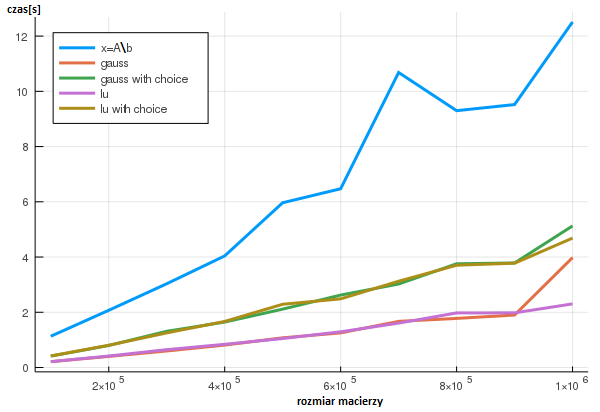
\includegraphics[width=0.90\textwidth]{plotwithlu.png}} \hfill
	\caption*{Wykres zależności czasu działania poszczególnych algorytmów od wielkości macierzy}
\end{figure}		

Widać, że standardowa implementacja metody eliminacji Gaussa w języku Julia (niebieski wykres) wypada najsłabiej. Inna obserwacja to fakt, że algorytmy bez wyboru elementu głównego (pomarańczowy i różowy) okazały się znacznie szybsze niż ich odpowiedniki, które wykonywały częściowy wybór elementu głównego (zielony i smutny żółty). Widać też, ze rozkład Gaussa (dla obu wariantów) działał w bardzo podobnym czasie co rozkład LU. Można z tego wyciągnąć wniosek, że rozkład Gaussa powinniśmy robić tylko w sytuacji jeśli jesteśmy całkowicie pewni, że będziemy musieli rozwiązać tylko jeden układ równań z daną macierzą. W innym przypadku warto zrobić rozkład LU, gdyż kosztuje nas to tylko niewiele więcej, a w przypadku konieczności rozwiązania innego układu równań gdzie zmieni się tylko wektor prawych stron, jesteśmy w stanie zrobić to już znacznie mniejszym nakładem pracy. Wykres pokazujący czasy rozwiązywania układu równań za pomocą rozkładu LU w zależności od wielkości macierzy znajduje się poniżej.
\clearpage

\begin{figure}[h]
	\centering
	\subfloat{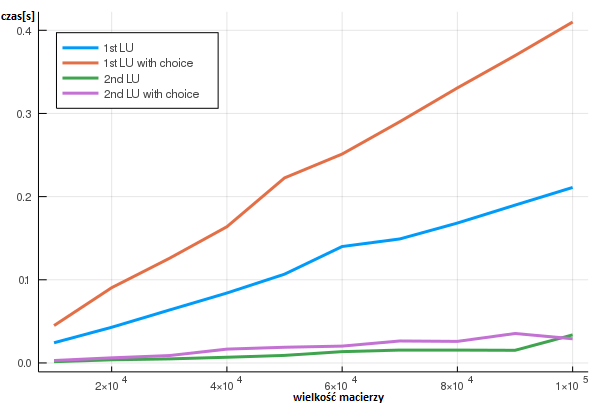
\includegraphics[width=1.0\textwidth]{luplot.png}} \hfill
	\caption*{Wykres zależności czasu rozwiązywanie układu równań za pomocą rozkładu LU od wielkości macierzy dla przypadku gdzie zrobiono to pierwszy raz oraz dla przypadku gdzie zrobiono to znając już rozkład LU danej macierzy.}
\end{figure}

Widać, że drugie (w praktyce oczywiście też kolejne) wywołanie funkcji rozwiązującej układ równań liniowych ze znanym już rozkładem LU zajęło znacznie mniej czasu niż rozwiązanie pierwsze wymagające jeszcze dodatkowo obliczenia rozkładu LU. Patrząc na wykresy można wyciągnąć wniosek, że to właśnie obliczanie rozkładu LU jest najbardziej kosztownym etapem algorytmu. Na tym wykresie widać również fakt zaobserwowany na poprzednim wykresie -- algorytmy, które nie wykonują wyboru elementu głównego są szybsze.

Dla wszystkich algorytmów zostały również obliczone błędy względne w przypadku kiedy wektor prawych stron $\vb$ był wyliczany. Macierze dla jakich wykonano eksperymenty miały wskaźnik uwarunkowania równy $10.0$, a $\ell=4$. Wyniki znajdują się w poniższej tabeli.

\begin{table}[!htbp]
	\centering
	\begin{tabular}{|c|c|c|}
		\hline
		rozmiar macierzy & gauss & gauss w wyborem   \\ \hline
		3000& $4.298823120065619\cdot 10^{-15}$ & $5.574749567941993\cdot 10^{-16}$   \\ \hline
		4000& $3.941408230930561\cdot 10^{-15}$ & $5.558576358655353\cdot 10^{-16}$    \\ \hline
		7000& $6.760775100733844\cdot 10^{-15}$ & $5.392236603514981\cdot 10^{-16}$  \\ \hline
		10000& $6.265367149198456\cdot 10^{-15}$ & $5.370519558488765\cdot 10^{-16}$ \\ \hline
	\end{tabular}
\end{table}

\begin{table}[!htbp]
	\centering
	\begin{tabular}{|c|c|c|}
		\hline
		rozmiar macierzy & lu & lu z wyborem  \\ \hline
		3000& $2.292966452680386\cdot 10^{-14}$ & $4.63979368199035\cdot 10^{-16}$  \\ \hline
		4000& $1.9944709360505984\cdot 10^{-14}$ & $ 4.576590595628056\cdot 10^{-16}$   \\ \hline
		7000& $1.5751008487442212\cdot 10^{-14}$ &$4.667824409854897\cdot 10^{-16}$ \\ \hline
		10000&$1.6235415592478852\cdot 10^{-14}$ & $4.582962454682111\cdot 10^{-16}$\\ \hline
	\end{tabular}
\end{table}

Widać, że algorytmy wykonujące częściowy wybór zwróciły dokładniejsze wyniki. Błąd względny w ich przypadku był rzędu $10^{-16}$. Dla porównania algorytmy, które nie wykonywały wyboru elementu głównego miały błędy rzędu $10^{-15}$ dla metody eliminacji Gaussa oraz $10^{-14}$ dla rozkładu LU.
\clearpage
Pierwszym wnioskiem z całej listy jest to, że zaimplementowane algorytmy faktycznie miały złożoność liniową (potwierdzają to również wykresy). Kolejny wniosek to fakt, że algorytmy dokonujące częściowego wyboru elementu głównego okazały się mieć większą złożoność, ale też zwracały dokładniejsze wyniki w odróżnieniu od algorytmów nie wykonujących wyboru. Zwróćmy też uwagę na fakt, że metody bez wyboru elementu głównego nie zadziałają w momencie kiedy na diagonali pojawi się element zerowy, zatem nie zawsze będzie możliwe ich użycie. Kolejny wniosek dotyczy rozkładu LU. Okazał się on bowiem wydajniejszy w przypadku kiedy rozwiązujemy wiele układów równań w których zmianie ulega tylko wektor prawych stron.
Kolejny wniosek to fakt, że dostosowanie reprezentacji danych pod konkretną ich strukturę może dać dużo większe możliwości. W tym przypadku była to możliwość przechowania macierzy rzędu nawet $10^6$ bez żadnego problemu. Standardowa reprezentacja macierzy nie dałaby takiej możliwości. Ponadto dzięki reprezentacji dobranej pod strukturę macierzy, ilość użytej pamięci była znacznie mniejsza. Ostatni wniosek to fakt, że dopasowanie algorytmów pod konkretną strukturę danych może znacznie przyspieszyć algorytm. W tym przypadku (również dzięki odpowiedniej reprezentacji macierzy w pamięci komputera) udało się \textit{zejść} ze złożoności $O(n^3)$ do złożoności liniowej, co jest znaczną poprawą.

\end{document}